\section{Lien avec les mathématiques discrètes}

\subsection{Permutations}

	\begin{tcolorbox}
		En mathématiques, la notion de \href{https://fr.wikipedia.org/wiki/Permutation}{permutation} exprime l'idée de réarrangement d'objets discernables. Une permutation d'objets distincts rangés dans un certain ordre correspond à un changement de l'ordre de succession de ces objets.
		\par
	\end{tcolorbox}

	On rappelle de fait qu'il existe $n!$ moyens d'ordonner $n$ éléments distincts.
	Considérons la permutation suivante qui envoie $1$ vers $4$, $2$ vers $1$, $3$ vers lui-même et $4$ vers $2$.

	\begin{center}
		\label{example1}
		$1 \longrightarrow 4$ \\
		$2 \longrightarrow 1$ \\
		$3 \longrightarrow 3$ \\
		$4 \longrightarrow 2$ \\
	\end{center}

	Il est tout à fait possible de représenter une permutation sous forme de graphe.

	\begin{center}
		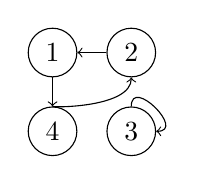
\begin{tikzpicture}[main/.style = {draw, circle}]
			\node[main] (1) {$1$};
			\node[main] (2) [right of=1] {$2$};
			\node[main] (4) [below of=1] {$4$};
			\node[main] (3) [below of=2] {$3$};

			\draw [arrows=->] (1) to (4);
			\draw[arrows=->] (4) .. controls +(up:3mm) and +(down:7mm) .. (2);
			\draw[->] (2) -- (1);
			\draw[->] (3) .. controls +(up:7mm) and +(right:7mm) .. (3);
			(3);
		\end{tikzpicture}
	\end{center}

	En voici un exemple plus poussé contenant 100 noeuds.

	\begin{center}
		\includegraphics[scale=0.4]{Figure_1}
	\end{center}

\subsection{Cycles d'une permutation}

	On souhaite maintenant considérer les cycles contenus dans les permutations.
	En continuant avec notre exemple, on remarque que notre permutation contient 2 cycles.
	Un cycle de longueur 3 $(1 \rightarrow 4 \rightarrow 2 \rightarrow 1)$ et un de longueur 1 $(3 \rightarrow 3)$.
	Sauf que, nous pouvons également remarquer que le cycle $(1 \rightarrow 4 \rightarrow 2 \rightarrow 1)$ est le même que $(4 \rightarrow 2 \rightarrow 1 \rightarrow 4)$ et $(2 \rightarrow 1 \rightarrow 4 \rightarrow 2)$. \\
	Il y a $3! = 6$ manières d'écrire une permutation de 3 éléments.
	Toutefois, on vient de dire qu'un cycle de 3 éléments pouvait s'écrire de 3 façons différentes; alors parmi ces $6$ permutations, il n'existe que $\frac{6}{3} = 2$ cycles distincts.
	\begin{align*}
		 & A \rightarrow B \rightarrow C \rightarrow A \qquad & A \rightarrow C  \rightarrow B \rightarrow A \\
		 & B \rightarrow C \rightarrow A \rightarrow B \qquad & C \rightarrow B  \rightarrow A \rightarrow C \\
		 & C \rightarrow A \rightarrow B \rightarrow C \qquad & B \rightarrow A  \rightarrow C \rightarrow B
	\end{align*}

	On peut le généraliser pour $n$ en disant qu'il y a $\frac{n!}{n} = (n-1)!$ façons d'écrire un cycle de $n$ éléments. \\

	On cherche maintenant à obtenir la quantité de permutations de $n$ contenant un cycle de longueur $ 0 < k \leq n$.
	Il y en a $\frac{n!}{k}$.

	\begin{align*}
		\binom{n}{k} * (k - 1)! * (n - k)! & = \frac{n!}{k! * (n - k)!} * (k - 1)! * (n - k)!           \\
		                                   & = \frac{n! * (k - 1)! * (n - k)!}{k * (k - 1)! * (n - k)!} \\
		                                   & = \frac{n!}{k}
	\end{align*}

	Avec
	\begin{itemize}
		\item $\binom{n}{k}$ : les éléments formant le cycle
		\item $(k - 1)!$ : le nombre de permutations des éléments formant le cycle
		\item $(n - k)!$ : le nombre de permutations des éléments restants
	\end{itemize}
